\begin{activite}[Aire d'un disque]
On a découpé des disques en parts égales (4 et 6) et disposé les morceaux ainsi.

\begin{center}
    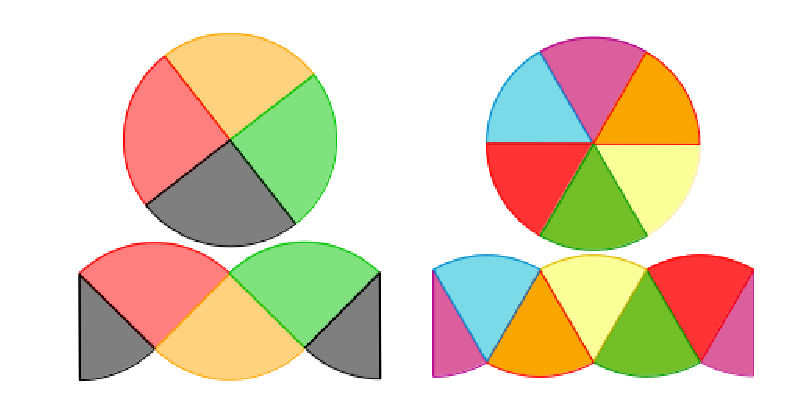
\includegraphics[width=.6\linewidth]{aCD01}
\end{center}

\begin{enumerate}
    \item Trace un disque de rayon 5\,cm. Partage-le en huit parts égales. Découpe-le et dispose‑le comme sur les exemples ci‑contre.
    \item De quelle forme se rapproche la figure reconstruite lorsque le nombre de parts augmente ?
    \item À quoi correspondent approximativement la largeur et la longueur de la figure pour le disque de départ ?
    \item Propose une méthode pour calculer l'aire du disque puis calcule l'aire d'un disque de rayon 10\,cm.
\end{enumerate}
\end{activite}



\begin{activite}[Formules et tableur]

\begin{partie}[Périmètre et aire d'un rectangle]
\begin{enumerate}
    \item Dans une feuille de calcul, reproduis ce tableau.
    \begin{center}
    \includegraphics[width=.66\linewidth]{aCD02}
    \end{center}
    \item Fais afficher dans la colonne \texttt{A} les nombres entiers pairs de 58 à 20, et dans la colonne \texttt{B} les nombres entiers de 1 à 20.
    \item Programme les cellules \texttt{C3} et \texttt{D3} pour qu'elles affichent les grandeurs demandées. Étire les formules jusqu'au dernier rectangle.
    \item Comment évolue le périmètre des rectangles ? 
    Comment évolue leur aire ? Pour quel rectangle l'aire est-elle maximale ? 
    \item Que dire du dernier rectangle ? Donne un autre rectangle de même aire que celui-ci.
\end{enumerate}
\end{partie}


\begin{partie}[Périmètre d'un cercle et aire d'un disque]
\begin{enumerate}
    \item Dans une nouvelle feuille de calcul, reproduis ce tableau.
    \begin{center}
    \includegraphics[width=.5\linewidth]{aCD03}
    \end{center}
    \item Fais afficher dans la colonne \texttt{A} les nombres entiers de 1 à 20. Programme les cellules \texttt{B3} et \texttt{C3} pour qu'elles affichent les grandeurs demandées (au centième près). Étire les formules jusqu'au dernier cercle.
 
    Quand on double le rayon d'un cercle, que se passe-t-il pour son périmètre ? 
    
    Quand on double le rayon d'un disque, que se passe-t-il pour son aire ?
\end{enumerate}
\end{partie}
\end{activite}



\begin{activite}[Découpages]
\ImageDroite{On considère un carré de côté 6\,cm composé de sept polygones particuliers comme l'illustre la figure ci-contre. On sait que le segment rouge mesure 2,2\,cm en vraie grandeur.}{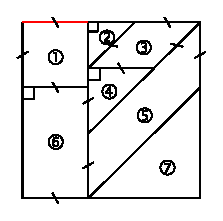
\includegraphics[width=.25\linewidth]{aCD04}}
\begin{enumerate}
    \item  Précise la nature de chaque polygone puis détermine son aire.
    \item Sur une feuille, construis en vraie grandeur le carré et découpe les sept pièces qui le constituent.
    \item En assemblant plusieurs de ces pièces, reconstitue chacune des figures suivantes et calcule leur aire.
    
    \vspace{1em}
    
    \ImageDroite{a)
    
    \includegraphics[width=.4\linewidth]{aCD05}}%
                {b)
                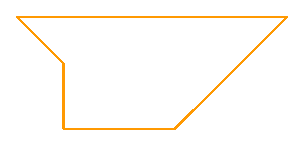
\includegraphics[width=.4\linewidth]{aCD06}}
    
\end{enumerate}

\end{activite}